% =============================================================================
% System view on the PYNQ-Z2: PS (ARM + DDR) <-> PL (interconnects, AXI DMA, accel)
% Shows GP0 vs HP0, control vs data paths, and the six steps of one Accel.run().
% Compile:  pdflatex pynq_system_dataflow.tex
% SVG:      pdftocairo -svg pynq_system_dataflow.pdf pynq_system_dataflow.svg
% =============================================================================
\documentclass[tikz,border=8pt]{standalone}
\usetikzlibrary{arrows.meta,positioning,calc,backgrounds}

\definecolor{ctrl}{HTML}{185FA5}   % AXI-Lite / control
\definecolor{data}{HTML}{C04828}   % bulk data (HP0, AXI-Stream)
\definecolor{cpu}{HTML}{5F5E5A}    % CPU <-> memory, clock/reset
\definecolor{ext}{HTML}{0F6E56}    % Xilinx IP
\definecolor{ours}{HTML}{993C1D}   % our design

\tikzset{
  >={Stealth[length=2.2mm]},
  blk/.style={draw, thick, rounded corners=2pt, align=center, inner sep=4pt, font=\small},
  ps/.style={blk, draw=cpu, fill=cpu!6},
  ip/.style={blk, draw=ext, fill=ext!7},
  acc/.style={blk, draw=ours, fill=ours!7},
  sig/.style={font=\scriptsize\ttfamily, inner sep=1.5pt},
  port/.style={sig, fill=white, draw, rounded corners=1pt},
  c/.style={->, very thick, draw=ctrl},
  d/.style={->, very thick, draw=data},
  k/.style={->, thick, draw=cpu},
  stp/.style={circle, draw=black, fill=yellow!35, inner sep=0.8pt, minimum size=4.2mm, font=\scriptsize\bfseries},
  ttl/.style={font=\small\bfseries, anchor=north west, inner sep=4pt},
}

\begin{document}
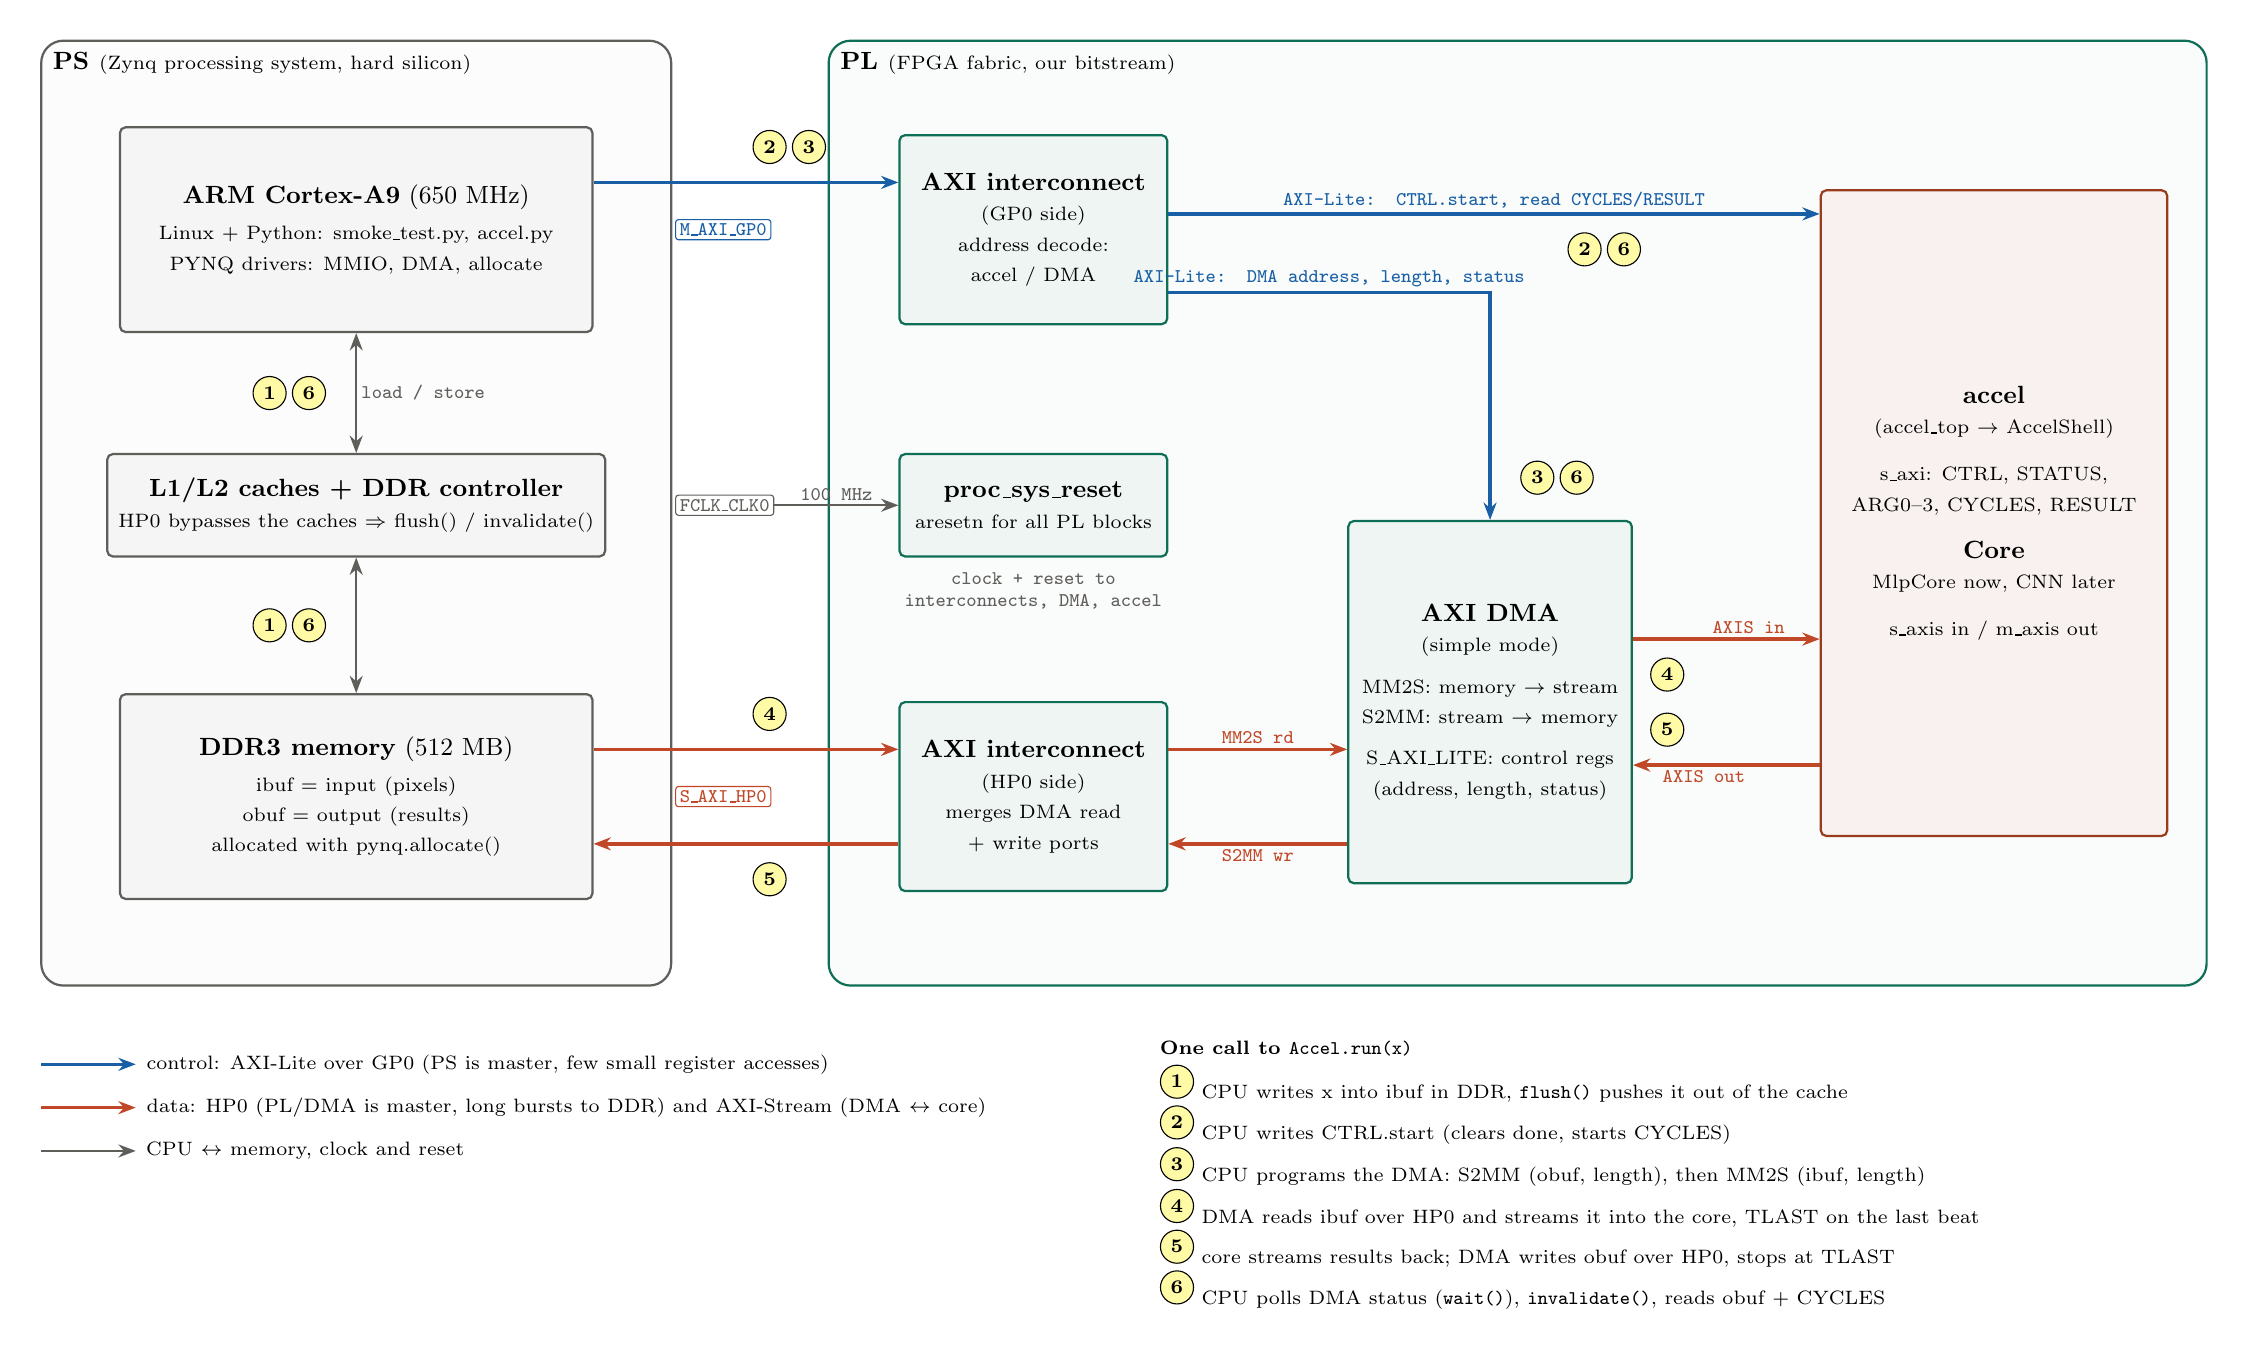
\begin{tikzpicture}[show background rectangle, background rectangle/.style={fill=white}]

% ---------------------------------------------------------------- containers
\draw[thick, rounded corners=8pt, draw=cpu, fill=cpu!2] (0,0) rectangle (8,12);
\node[ttl] at (0,12) {PS \normalfont\scriptsize(Zynq processing system, hard silicon)};
\draw[thick, rounded corners=8pt, draw=ext, fill=ext!2] (10,0) rectangle (27.5,12);
\node[ttl] at (10,12) {PL \normalfont\scriptsize(FPGA fabric, our bitstream)};

% ---------------------------------------------------------------- PS contents
\node[ps, minimum width=6cm, minimum height=2.6cm] (arm) at (4,9.6)
  {\textbf{ARM Cortex-A9} (650 MHz)\\[2pt]\scriptsize Linux + Python: smoke\_test.py, accel.py\\\scriptsize PYNQ drivers: MMIO, DMA, allocate};
\node[ps, minimum width=6cm, minimum height=1.3cm] (cache) at (4,6.1)
  {\textbf{L1/L2 caches + DDR controller}\\\scriptsize HP0 bypasses the caches $\Rightarrow$ flush() / invalidate()};
\node[ps, minimum width=6cm, minimum height=2.6cm] (ddr) at (4,2.4)
  {\textbf{DDR3 memory} (512 MB)\\[2pt]\scriptsize ibuf = input (pixels)\\\scriptsize obuf = output (results)\\\scriptsize allocated with pynq.allocate()};

\draw[k, <->] (arm.south) -- (cache.north) node[midway, right, sig, text=cpu] {load / store};
\draw[k, <->] (cache.south) -- (ddr.north);
\node[stp] at ($(arm.south)!0.5!(cache.north)+(-1.1,0)$) {1};
\node[stp] at ($(arm.south)!0.5!(cache.north)+(-0.6,0)$) {6};
\node[stp] at ($(cache.south)!0.5!(ddr.north)+(-1.1,0)$) {1};
\node[stp] at ($(cache.south)!0.5!(ddr.north)+(-0.6,0)$) {6};

% ports on the PS/PL boundary
\node[port, draw=ctrl, text=ctrl, anchor=west] (gp0) at (8.05,9.6) {M\_AXI\_GP0};
\node[port, draw=data, text=data, anchor=west] (hp0) at (8.05,2.4) {S\_AXI\_HP0};
\node[port, draw=cpu,  text=cpu,  anchor=west] (fclk) at (8.05,6.1) {FCLK\_CLK0};

% ---------------------------------------------------------------- PL contents
\node[ip, minimum width=3.4cm, minimum height=2.4cm] (gpic) at (12.6,9.6)
  {\textbf{AXI interconnect}\\\scriptsize (GP0 side)\\\scriptsize address decode:\\\scriptsize accel / DMA};
\node[ip, minimum width=3.4cm, minimum height=1.3cm] (rst) at (12.6,6.1)
  {\textbf{proc\_sys\_reset}\\\scriptsize aresetn for all PL blocks};
\node[ip, minimum width=3.4cm, minimum height=2.4cm] (hpic) at (12.6,2.4)
  {\textbf{AXI interconnect}\\\scriptsize (HP0 side)\\\scriptsize merges DMA read\\\scriptsize + write ports};

\node[ip, minimum width=3.6cm, minimum height=4.6cm] (dma) at (18.4,3.6)
  {\textbf{AXI DMA}\\\scriptsize (simple mode)\\[4pt]\scriptsize MM2S: memory $\to$ stream\\\scriptsize S2MM: stream $\to$ memory\\[4pt]\scriptsize S\_AXI\_LITE: control regs\\\scriptsize (address, length, status)};

\node[acc, minimum width=4.4cm, minimum height=8.2cm] (accel) at (24.8,6.0)
  {\textbf{accel}\\\scriptsize (accel\_top $\to$ AccelShell)\\[6pt]\scriptsize s\_axi: CTRL, STATUS,\\\scriptsize ARG0--3, CYCLES, RESULT\\[6pt]\textbf{\small Core}\\\scriptsize MlpCore now, CNN later\\[6pt]\scriptsize s\_axis in / m\_axis out};

% ---------------------------------------------------------------- control paths (blue)
\draw[c] (arm.east |- 0,10.2) -- (gpic.west |- 0,10.2);
\node[stp] at (9.25,10.65) {2};
\node[stp] at (9.75,10.65) {3};
\draw[c] (gpic.east |- 0,9.8) -- (accel.west |- 0,9.8)
  node[sig, pos=0.5, above, text=ctrl] {AXI-Lite: CTRL.start, read CYCLES/RESULT};
\node[stp] at (19.6,9.35) {2};
\node[stp] at (20.1,9.35) {6};
\draw[c] (gpic.east |- 0,8.8) -| (dma.north)
  node[sig, pos=0.25, above, text=ctrl] {AXI-Lite: DMA address, length, status};
\node[stp] at (19.0,6.45) {3};
\node[stp] at (19.5,6.45) {6};

% ---------------------------------------------------------------- data paths (red)
\draw[d] (ddr.east |- 0,3.0) -- (hpic.west |- 0,3.0);
\draw[d] (hpic.west |- 0,1.8) -- (ddr.east |- 0,1.8);
\node[stp] at (9.25,3.45) {4};
\node[stp] at (9.25,1.35) {5};

\draw[d] (hpic.east |- 0,3.0) -- (dma.west |- 0,3.0) node[sig, midway, above, text=data] {MM2S rd};
\draw[d] (dma.west |- 0,1.8) -- (hpic.east |- 0,1.8) node[sig, midway, below, text=data] {S2MM wr};

\draw[d] (dma.east |- 0,4.4) -- (accel.west |- 0,4.4) node[sig, pos=0.62, above, text=data] {AXIS in};
\draw[d] (accel.west |- 0,2.8) -- (dma.east |- 0,2.8) node[sig, pos=0.62, below, text=data] {AXIS out};
\node[stp] at (20.65,3.95) {4};
\node[stp] at (20.65,3.25) {5};

% ---------------------------------------------------------------- clock / reset (gray)
\draw[k] (fclk.east) -- (rst.west) node[sig, midway, above, text=cpu] {100 MHz};
\node[sig, text=cpu, align=center, anchor=north] at (12.6,5.3) {clock + reset to\\interconnects, DMA, accel};

% ---------------------------------------------------------------- legend + steps
\begin{scope}[shift={(0,-1.0)}]
  \draw[c] (0,0) -- (1.2,0) node[right, font=\scriptsize, text=black] {control: AXI-Lite over GP0 (PS is master, few small register accesses)};
  \draw[d] (0,-0.55) -- (1.2,-0.55) node[right, font=\scriptsize, text=black] {data: HP0 (PL/DMA is master, long bursts to DDR) and AXI-Stream (DMA $\leftrightarrow$ core)};
  \draw[k] (0,-1.1) -- (1.2,-1.1) node[right, font=\scriptsize, text=black] {CPU $\leftrightarrow$ memory, clock and reset};
\end{scope}

\node[anchor=north west, font=\scriptsize, align=left, inner sep=0pt] at (14.2,-0.7) {%
  \textbf{One call to \texttt{Accel.run(x)}}\\[2pt]
  \tikz\node[stp]{1}; CPU writes x into ibuf in DDR, \texttt{flush()} pushes it out of the cache\\
  \tikz\node[stp]{2}; CPU writes CTRL.start (clears done, starts CYCLES)\\
  \tikz\node[stp]{3}; CPU programs the DMA: S2MM (obuf, length), then MM2S (ibuf, length)\\
  \tikz\node[stp]{4}; DMA reads ibuf over HP0 and streams it into the core, TLAST on the last beat\\
  \tikz\node[stp]{5}; core streams results back; DMA writes obuf over HP0, stops at TLAST\\
  \tikz\node[stp]{6}; CPU polls DMA status (\texttt{wait()}), \texttt{invalidate()}, reads obuf + CYCLES};

\end{tikzpicture}
\end{document}
